\chapter{Perceptron}
\label{ch:perceptron}
Perceptrons are among KNN and NCC one of the simplest, yet powerful and popular algorithms. They are the easiest form of Neural Networks
that we know of and are a great introduction into the field of Artificial Neural Networks.

But first we make a small recap of the NCC algorithm. Remember, we defined the prototypes corresponding to each class as the means
\begin{align}
  \vec{\mu}_{\triangle} = \frac{1}{N_{\triangle}} \sum_{\vec{x} \in \mathcal{X}_{\triangle}} \vec{x}\\
  \vec{\mu}_{\circ} = \frac{1}{N_{\circ}} \sum_{\vec{x} \in \mathcal{X}_{\circ}} \vec{x}
\end{align}
to classify a new data point $\vec{x}$ we saw that we must compute the distance to each class mean.
For the example in Figure \ref{fig:prototypes_2} this translates to
\begin{equation}
  \text{d}(\vec{x}, \vec{\mu}_{\triangle}) > \text{d}(\vec{x}, \vec{\mu}_{\circ})
\end{equation}
After several steps of rearranging the definitions of both sides, we ended up with
\begin{equation}
  0 > \left(\vec{\mu}_{\circ} - \vec{\mu}_{\triangle}\right)^T \vec{x} + \frac{1}{2} \left(\vec{\mu}_{\triangle}^T \vec{\mu}_{\triangle} - \vec{\mu}_{\circ}^T \vec{\mu}_{\circ}\right)
\end{equation}
That can be transformed into the general form of a linear classifier
\begin{equation}
  \vec{w}^T \vec{x} + \beta = \left\{\begin{matrix}
    > 0 \text{ if } \vec{x} \text{ belongs to class } \triangle\\
    < 0 \text{ if } \vec{x} \text{ belongs to class } \circ
  \end{matrix}\right.
\end{equation}
For NCC we defined $\vec{w}$ to be the difference vector of the class means $\left(\vec{\mu}_{\circ} - \vec{\mu}_{\circ}\right)$ and $\beta$ some constant offset.
This class of linear classifiers is super important in Machine Learning, especially if we want to perform classifications fast and efficiently. A lot of technologies that must perform
fast classifications are using those linear classification algorithms, something like a perceptron.

We will briefly recall the visual representation of linear classifiers as showcased in Figure \ref{fig:linear_classifier_origin_bias}.
For a new data point $\vec{x}$ we can assign a class label by projecting $\vec{x}$ onto $\vec{\omega}$ via $\vec{\omega}^T \vec{x}$.
If this resulting scalar is bigger than the threshold $\beta$, we assign the class label $\triangle$, otherwise $\circ$.
Now, if we would classify a lot of samples we might see a distribution showcased in Figure \ref{fig:lin_classifier_distribution} for $\circ$ like the grey line and for $\triangle$ like the orange one.


\begin{figure}[h]
  \centering
  \includegraphics[width=0.5\textwidth]{figures/lin_classifier_distribution.png}
  \caption{Distribution of the class labels $\triangle$ and $\circ$ for a linear classifier.}
  \label{fig:lin_classifier_distribution}
\end{figure}

In the previous chapter we saw that this $\beta$ threshold would be "perfect", but we might want to optimize for a different metric, for instance precision or recall, which would adjust the threshold.

Good, now that we refreshed our knowledge on linear classifiers, we can move on to the perceptron.

We know linear classifiers predict classes and what they are. But we didn't answer yet how to calculate the parameters $\vec{\omega}$ and $\beta$ in a general way, how can we find this vector efficiently?

From the NCC algorithm we remember there's a very simple way to compute $\vec{\omega}$, namely the difference vector of the class means. And we learned in the NCC chapter that this method
restricts the algorithm vastly and has several drawbacks.

Usually, the computation of $\vec{\omega}$ is done a little different for general linear classificators. Instead of coming up with a definition to compute $\vec{\omega}$, we must define a so called \textit{error}/\textit{loss function}.

\section{Error Functions}
Error functions are functions of the group $\Epsilon(\vec{x}, \vec{y}, \vec{\omega})$.
Given data points $\vec{x} \in \mathbb{R}^d$ and their corresponding class labels $\vec{y} \in \mathbb{R}^{d_y}$ and a vector of parameters $\vec{\omega} \in \mathbb{R}^d$
it computes the error of our model with the given weights $\vec{\omega}$ on the data points $\vec{x}$.

For now and the rest of this chapter we will assume to only have binary labels, e.g. $\vec{y} \in \left\{-1, 1\right\}$. This is not a big restriction, since we can always transform
any multi-class problem into a binary one by using the one-vs-all approach that we will see at the end of this chapter (Section \ref{sec:combining_perceptrons}).

There are two very popular error functions that we will discuss in this chapter, namely the \textit{Square Error} (Adaline Loss) and the \textit{Perceptron Loss}.

\begin{table}[h]
  \centering
  \begin{tabular}{|l|l|}
    \hline
    \textbf{Error Function} & \textbf{Definition}\\
    \hline
    Square Error & $\Epsilon(\vec{x}, \vec{y}, \vec{\omega}) = \frac{1}{2} \left(\vec{y} - \vec{\omega}^T \vec{x}\right)^2$\\
    \hline
    Perceptron Loss & $\Epsilon(\vec{x}, \vec{y}, \vec{\omega}) = \max\left(0, -\vec{y} \vec{\omega}^T \vec{x}\right)$\\
    \hline
  \end{tabular}
  \caption{Error functions for linear classifiers.}
  \label{tab:error_functions}
\end{table}
The table \ref{tab:error_functions} shows the two error functions that we will discuss in this chapter. The first one is the square error, also known as Adaline loss. The second one is the perceptron loss.

\section{Rosenblatt's Perceptron}
The second error function was invented by Frank Rosenblatt (Figure \ref{fig:rosenblatt}) in 1957.
He was the inventor of the Perceptron algorithm and is therefore the creator of the field of ANNs.

\begin{minipage}{0.45\textwidth}
\begin{figure}[h]
  \centering
  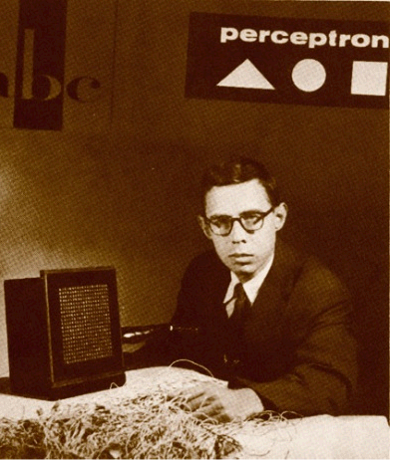
\includegraphics[width=0.5\textwidth]{images/rosenblatt.jpg}
  \caption{Frank Rosenblatt, inventor of the perceptron.}
  \label{fig:rosenblatt}
\end{figure}
\end{minipage}
\hfill
\begin{minipage}{0.45\textwidth}
\begin{quote}
He studied perceptrons, so that the fundamental laws of organization which are common to all information handling systems, machines and men included, may eventually be understood
\end{quote}
- quite a bold statement.
\end{minipage}

We will now briefly introduce ANNs, but we will go into more detail later, in Chapter \ref{ch:neural-networks}.
\subsection{Artificial Neural Networks}
Rosenblatt was influenced in his ANN architecture design by human brains. His implementation is a very, very simplified computational model that uses some aspects of their biological role model.
An ANN consists of \textit{input neuros} ($x_1, x_2, \dots$) that are weighted with corresponding \textit{synaptic weights} ($w_1, w_2, \dots$).
The sum of these weighted inputs is then used to compute the prediction.
The method $f(...)$ is a non-linear function, that we omit for now, which will decide upon the final label
\begin{equation}
  f(\vec{x}) = \left\{\begin{matrix}
    1 \text{ if } \vec{x} \text{ is preferred stimulus}\\
    -1 \text{ otherwise}
  \end{matrix}\right.
\end{equation}

You can see a visualization of such Perceptron in Figure \ref{fig:perceptron}.

\begin{figure}[h]
  \centering
  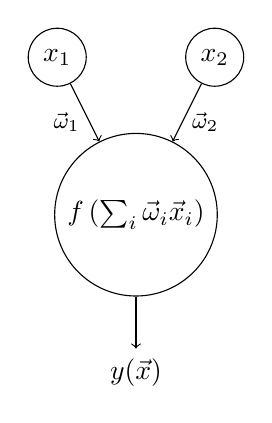
\begin{tikzpicture}
    \node[draw, circle] (x1) at (0, 0) {$x_1$};
    \node[draw, circle] (x2) at (2, 0) {$x_2$};
    \node[draw, circle] (x3) at (1, -2) {$f\left(\sum_i \vec{\omega}_i \vec{x}_i\right)$};
    \node (x4) at (1, -4) {$y(\vec{x})$};

    \draw[->] (x1) -- (x3) node [pos=0.66,left,font=\footnotesize] {$\vec{\omega}_1$};
    \draw[->] (x2) -- (x3) node [pos=0.66,right,font=\footnotesize] {$\vec{\omega}_2$};
    \draw[->] (x3) -- (x4);
  \end{tikzpicture}
  \caption{Visualization of a Perceptron.}
  \label{fig:perceptron}
\end{figure}
This is pretty abstract now, but apart from the non-linear function $f(...)$, this is exactly what we saw in the previous chapter.

When Rosenblatt implemented his Perceptron it required a full room of hardware, with massive mechanical relays and giant memory rigs.
Nowadays, we can run the perceptron algorithm on a microcontroller, or even on a small chip that is capable of matrix-vector multiplication.
The original Perceptron algorithm was used to classify handwritten text, we will use exactly the same use case to showcase the algorithm.

\section{The Perceptron Learning Algorithm}
Now we will look deeper into the Perceptron algorithm.
The goal is to perform binary classification of multivariate data points $\vec{x} \in \mathbb{R}^d$.

The input for the algorithm are $N$ tuples of data points $\vec{x}_i$ and their corresponding class labels $y_i$, where $y_i \in \left\{-1, 1\right\}$, such that
\begin{align}
  y_n = \left\{\begin{matrix}
    1 \text{ if } \vec{x}_n \text{ belongs to class }\
    -1 \text{ if } \vec{x}_n \text{ does not belong to class }
  \end{matrix}\right.
\end{align}
additionally the algorithm receives a parameter called \textit{learning rate} $\eta$, we will define this in a second.

The output of the algorithm is a vector of weights $\vec{\omega}$ and a bias $\beta$ that define the linear classifier
\begin{align}
  \vec{\omega}^T \vec{x} + \beta = \left\{\begin{matrix}
    \geq 0 \text{ if } y_n = +1\\
    < 0 \text{ if } y_n = -1
  \end{matrix}\right.
\end{align}
Recall the optimization note in the NCC lecture, where we learned that we can also write $\beta$ into $\vec{\omega}$ by adding a constant dimension to $\vec{x}$
\begin{equation}
  \vec{\hat{\omega}} = \left[\beta,\vec{\omega}\right]^T, \vec{\hat{x}} = \left[1, \vec{x}\right]^T
\end{equation}

\ssection{The Perceptron Error Function}
This is a reformulation of the perceptron loss function from Table \ref{tab:error_functions}
\begin{equation}
  \Epsilon(\vec{x}, y, \vec{\omega}) = \max\left(0, -y \vec{\omega}^T \vec{x}\right) = -\sum_{m \in \mathcal{M}} \vec{\omega}^T \vec{x}_m y_m
\end{equation}
where $\mathcal{M}$ is the set of all misclassified data points.

\subsection{Classification Error as Function of weights}
You can see a plot of this error function in Figure \ref{fig:perceptron_error_function}. On the left side we have all correct classified labels, on the right the misclassified ones.

Now, let's look at a real 2D example data set. On the right side you can see a plot for the error, if we project our $\vec{\omega}$ vector onto any point in our coordinate system on the left side.

So each point on the right grid represents a potential $\vec{\omega}$ vector. The color of the point represents the error of this $\vec{\omega}$ vector.
To find the best value for $\vec{\omega}$ we must find the minimum of this error function. But usually we can't just simply create this plot, nor can we try out every possible value for $\vec{\omega}$ in finite time.
So in general, what we do in ML is, to randomly initialize $\vec{\omega}$ and evaluate our error function. But instead of evaluating the regular error function, we evaluate it's gradient.
This gives us the steepness of the error function in $\vec{\omega}$. To minimize the error through $\vec{\omega}$ we then adjust $\vec{\omega}$ in the opposite direction of the gradient.
This works, because the gradient of the error function points into the direction of the biggest error.
This process is called \textit{Gradient Descent (GD)} and is a very popular optimization technique in ML.
\section{Gradient Descent}
\label{sec:gradient_descent}
Gradient Descent is, as we just saw, an algorithm that can optimize a function $f(\vec{x}, \vec{\omega})$ by iteratively adjusting the parameters $\vec{\omega}$ in the opposite direction of the gradient of $f$. Hence we can use GD to minimize the error function of the Perceptron algorithm.

We randomly initialize $\vec{\omega}$ and then iteratively update it by subtracting the gradient of the error function $\Epsilon(\vec{x}, y, \vec{\omega})$.
And this is how GD works in detail
We have an old value for $\vec{\omega}$, $\vec{\omega}^{\text{old}}$, e.g. randomly initialized, compute the gradient of the error function using $\vec{\omega}^{\text{old}}$ by summing over all training samples that is scaled by $\eta$, the learning rate, to compute
\begin{equation}
  \vec{\omega}^{\text{new}} = \vec{\omega}^{\text{old}} - \eta \sum_{i=1}^{X} \nabla_{\vec{\omega}} \Epsilon(\vec{x}, y, \vec{\omega})
\end{equation}
Here you can see why this algorithm is called GD, we subtract the current gradient from our current weights. The learning rate $\eta$ determines how fast we descent.
The resulting $\vec{\omega}^{\text{new}}$ will be the new adjusted weights from our model. We can now repeat this process until we reach a certain threshold in the error, or until we reach a certain number of iterations.

\subsection{Stochastic Gradient Descent}
\subsection{Mini-Batch Gradient Descent}

\section{Perceptron Training}
\section{Problems with the Perceptron Algorithm}
\section{Application Example: Handwritten Digits}
\section{Derivation of the Perceptron Error Function}

\section{Combining multiple Perceptrons}
\label{sec:combining_perceptrons}

\subsection{One-vs-All}
\subsection{One-vs-One}

\subsection{Application Example: Handwritten Digits (multi-class)}

\framedtext{\color{red}{TODO:}}

